% ===============================================================
%
%  Template for creating scribe notes for CS:3330, Algorithms.             I am using this template to get my homework PDF's set up as well
%
%  Fill in your name, lecture date, and body of scribe notes
%  as indicated below.
%
% ===============================================================

\documentclass[11pt]{article}

\usepackage{graphicx}
\usepackage{amssymb, amsthm}
\usepackage{pgfplots}
\usepackage{tikz}
\usetikzlibrary{datavisualization}
\usetikzlibrary{datavisualization.formats.functions}
\usepackage{mathtools}
\usepackage{amsmath}
\usepackage{algorithmicx}
\usepackage{algorithm}
\usepackage{algpseudocode}
\usepackage{multirow}



\setlength{\topmargin}{0pt}
\setlength{\textheight}{9in}
\setlength{\headheight}{0pt}
\setlength{\headsep}{0pt}
\setlength{\oddsidemargin}{0.25in}
\setlength{\textwidth}{6in}

\pagestyle{plain}

\begin{document}

\thispagestyle{empty}

\begin{center}
\bf\large CS:3330, Algorithms
\end{center}

\begin{center}
\bf\large HW12 - SSSP  %Fill in Name of Homework here
\end{center}

\noindent
Logan Zweifel     % FILL IN YOUR NAME HERE
\hfill
November, 7 2021           % FILL IN HW DATE HERE

\noindent
\rule{\textwidth}{1pt}

\medskip

%%%%%%%%%%%%%%%%%%%%%%%%%%%%%%%%%%%%%%%%%%%%%%%%%%%%%%%%%%%%%%%%
% BODY OF HOMEWORK NOTES GOES HERE
%%%%%%%%%%%%%%%%%%%%%%%%%%%%%%%%%%%%%%%%%%%%%%%%%%%%%%%%%%%%%%%%



\section{Dijksta's 1}
Suppose Dijkstra's SSSP algorithm is run on the below graph

\begin{center}
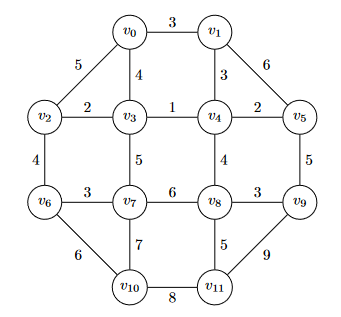
\includegraphics{Q1.png}
\end{center}

\subsection*{a) Show the contents of D}

\bigskip
\bigskip
\begin{center}
$D = [0, 3, 5, 4, 5, 7, 9, 9, 9, 12, 15, 14]$
\end{center}

\bigskip
\bigskip

\subsection*{b) show the contents of P}

\bigskip
\bigskip

\begin{center}
$P = [0, 0, 0, 0, 3, 4, 2, 3, 4, 5, 6, 8]$
\end{center}



\section{Dijksta's 2}
Suppose Dijkstra's SSSP algorithm return the following D and P for sime input graph G.\\
\noindent $D = [0, 30, 32, 2, 8, 10, 5, 7, 18]$ \\
\noindent $P = [0, 0, 1, 0, 7, 0, 3, 6, 5]$

\bigskip
\bigskip

\subsection*{a) How many vertices are in G?}

\bigskip
\bigskip
\begin{center}
There are 9 vertices
\end{center}

\bigskip
\bigskip

\subsection*{b) What is the shortest bath from $v_0$ to $v_4$}

\bigskip
\bigskip
\begin{center}
$\{ v_0, v_3, v_6, v_7, v_4 \}$
\end{center}

\bigskip
\bigskip

\subsection*{c) What is the weight of the shortest path from $v_0$ to $v_2$}

\bigskip
\bigskip

\begin{center}
The weight of the shortest path from vertex 0 to vertex 2 is 32
\end{center}





























%%%%%%%%%%%%%%%%%%%%%%%%%%%%%%%%%%%%%%%%%%%%%%%%%%%%%%%%%%%%%%%%

\end{document}

